\section{Agents}
% rewrite to match the current system

As mentioned before, there are two main types of agents: generators and testers.
Generators extend or modify an existing counterpoint line to create a new partial composition.
Testers examine a counterpoint line (usually at the current end) to see if it acceptable.

% moved to System Design
%Generators and testers work together through a feedback loop to create valid compositions.
%
%\begin{figure}[h]
%\centering
	%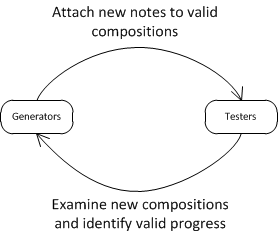
\includegraphics[keepaspectratio=true]{generator-and-tester-dynamic.png}
%\caption{The generator and tester agent dynamic}
%\end{figure}

Agents can also be divided by the ruleset they help implement. 
In this case, there are general counterpoint rules that apply to all species of counterpoint, and there are first species specific rules.
%For example, implementing florid counterpoint involves six rulesets: general rules, four sets of species specific rules, and species boundary rules.

Regarding counterpoint, tester agents have another division: hard rules (mandatory) and soft rules (optional, but preferred).
These rules were derived from the descriptions in ``Modal Counterpoint: Renaissance Style'' by Peter Schubert. % TODO(add better citation later).

\subsection{General Counterpoint Rules}

\paragraph{Generators}
The form of a note depends upon the counterpoint species, so there is no reasonable way to generate notes outside the context of a species.
Therefore, general counterpoint has no generators.
%The counterpoint species determines the start and duration of a note, so there is no reasonable way to generate notes outside of the context of a species.
%Thus, no generator agents fall within the General Counterpoint Rules grouping.

\paragraph{Testers}
\subparagraph{Hard Rules}
	\begin{enumerate}
		\item No augmented or diminished skips. No skips larger than a sixth unless it is an octave.
					Implementation involves checking the current and previous notes to build the interval and test it.

		\item The first and last notes of each part (\emph{cantus firmus} and counterpoint) must form a perfect consonant interval, i.e. a perfect unison, fifth, octave, or occasionaly a twelth.
          The implementation of this rule automatically passes interior notes.

		\item No outlines of augmented fourths. No outlines of diminished fifths unless completely filled in and followed by an opposite direction step.
          A note is a temporary high note if it is higher than both notes adjacent to it. A temporary low note is similarly defined.
          An interval is outlined if a temporary high note and a temporary low note (with no other temporary highs or lows in between) form that interval.
					Implementation involves moving back from the current note to find the last complete segment with a low and a high, and then testing that interval.
					Testing the segment ending in the current note does not serve much purpose because we don't know if it will be a local high or low yet. The exception is the last note of the composition.

	\end{enumerate}
\subparagraph{Soft Rules}
	\begin{enumerate}
		%\item Use steps, movement to adjacent notes, more than skips, movement to non-adjacent notes. Specific ratios are usually determined by species, but the general agent would aim for a minimum rate.
		
		\item Avoid skips of a major sixth and descending minor sixths. The implementation only needs to check the interval of the current note and the preceding note.

		\item Precede or follow a skip by a step in the opposite direction. Examine the current note and the two preceding notes in order to check validity of the first preceding note.

		\item Do not use more than two skips in sequence. Examine the current note and the three preceding notes to check if all three intervals are skips.

		\item Two successive skips in the same direction should be small skips. A `small' interval is a fourth or smaller. Check the two most recent intervals.

		\item In a sequence of skips and steps in the same direction, larger intervals should be below smaller ones.
          The implementation examines the two most recent intervals. If they are both motions in the same direction, it tests if the larger interval is below the smaller interval.

		\item Do not skip both to and from a high or low point. Scan back to the previous high or low and check if it is bounded by skips on both sides.

	\end{enumerate}

\subsection{First Species Counterpoint Rules}

First species involves matching each note of the \emph{cantus firmus} with one simultaneous note of counterpoint.
Since the \emph{cantus firmus} is typically written using whole notes, first species also uses whole notes.

\paragraph{Generators}
The basic first species generator randomly selects a note within and octave up or down from the most recent note of the counterpoint and attaches to the end of the counterpoint.
For the first note, the generator uses the first note of the \emph{cantus firmus} since there is no note in the counterpoint to work from.
The attached note also has a random accidental. The accidental is limited to at most one, so the only possibilities are one flat, a natural, or one sharp.

\paragraph{Testers}
All first species testers check whether the current note meets the criteria of first species counterpoint. If it is not, the rule automatically passes.
This enables rules for different species to be mixed while only enforcing relevant rules.
\subparagraph{Hard Rules}
	\begin{enumerate}
		\item All downbeats, which in the case of first species is all beats, must be consonant with the \emph{cantus firmus}. 
					Consonant intervals are unisons, thrids, fifths, sixths, octaves, and their compounds.
					This agent just checks the current note with the corresponding note in the \emph{cantus firmus}.

		\item Enter perfect intervals only by contrary motion, in which voices move in opposite directions, or oblique motion, in which one voice does not move.
					If the current vertical interval is perfect, then the agent examines the motion from the previous notes in both voices.

		\item Both voices may not repeat their previous note at the same time. Either voice may repeat the previous note, but not both simultaneously.
          The implementation examines the most recent interval in each voice and examines if at least one is not a unison.

		\item The counterpoint and the \emph{cantus firmus} can move in parallel (same vertical interval) for at most four notes.
          The implementation examines the four most recent vertical intervals and checks that they are not all equal.

		\item Skips must be less than half of all melodic motions in the counterpoint.
          This agent counts the number of skips in the counterpoint up to the current note and the total number of motions in the \emph{cantus firmus}.
          If the number of skips so far is less than half the total number of \emph{cantus firmus} motions, then the test passes.

	\end{enumerate}
\subparagraph{Soft Rules}
	\begin{enumerate}
		\item Avoid using more that two perfect vertical intervals in a row. This agent just checks the two most recent vertical intervals to test if at least one is not perfect.
		\item Avoid vertical unisons except on the first and last notes. If the current note is not the first or last note, then the agent tests whether the vertical interval is a unison.
		\item Avoid simultaneous skips. It is ok if both voices are skipping by a third. This agent checks the most recent interval in both voices and checks if both are large skips.
		\item Avoid the vertical interval being larger than a twelfth. This agent only checks the current vertical interval.
	\end{enumerate}
